\section{Introduction} \label{sec:intro}


Remote sensing technology is an important source of Earth observation from different platforms
and sensors, and it offers to work on a large scale with cheap, fairly accurate, and faster results compared to ground-based methods.

Land Surface Temperature (LST) images at a high temporal resolution are of prime importance to efficiently monitor physical processes related to climate change such as water stress, evapotranspiration, risk of wildfires or urban heat islands \cite{lst2005}.
Additionally, LST has been approved as one of the high-priority parameters for the International Geosphere and Biosphere Program (IGBP) \cite{townshend94}.

LST is retrieved from remote sensing images in the Thermal infra-red (TIR) spectral domain.  
Some of the applications mentioned before have very exigent requirements for the TIR data products, needing as many detailed images as possible (spatial resolution), but also having as many images available per day to monitor such dynamic processes (temporal resolution).
Unfortunately, these requirements are not met by the currently available products and research may be hindered by the lack of data.

Upcoming missions such as SBG, Trishna and LSTM will join forces to provide a 50m GSD product at daily revisit \cite{author2023thermal}. However, their full joint system will not be available until end of the current decade assuming there are no further delays. Additionally, applications like urban heat require more than one image per day.
Private satellite providers such as OroraTech are deploying constellations of smaller satellites that provide very high temporal resolution, but their smaller payload generally result in lower spatial resolution that is not enough for local scale applications and fine scale analysis, especially for highly heterogeneous environments like urban areas, diverse agricultural plots or sparse forests.

Super resolution (SR) is a post-processing technique that aims to increase the spatial resolution of images while preserving their physical consistency.
Using artificial intelligence (AI) for SR has many applications in heterogeneous fields like medical imaging, computer vision and also remote sensing. 

While several deep learning architectures have been proposed with promising results in synthetic datasets, it remains a challenge to apply them to real data.
This is because most of the assumptions made to generate the datasets needed for training do not represent the physical reality accurately.
Throughout this thesis, super resolution of TIR data products provided by OroraTech's mission FOREST-2 will be explored, so that better LST products can be developed and improvements in research may be achieved.
Additionally, the impact of the degradation models used for dataset generation will be studied, and a framework that allows SR from low spatial resolution TIR data products coming from any mission will be proposed.
 
In Chapter 2, a brief introduction to remote sensing and LST retrieval is presented, alongside of dimensions of quality of remote sensing data.

In Chapter 3, the motivation of this work is presented, diving deeper into applications of TIR data and their requirements.
The trade-off between spatial and temporal resolution that the current available products is also shown, making it the main driver super-resolution.

The main techniques of super resolution are presented in Chapter 4, as well as the main challenges in dataset generation techniques used in the literature.
The domain gap problem is also introduced, as well as the concept of blind super-resolution.

In Chapter 5, the methodology of this work is presented, including the models architecture and the rationale behind their selection. Additionally, the degradation models used to obtain a baseline model and the metrics used for evaluation are discussed.

In Chapter 6, the data gathering process is introduced and the datasets that will be used in the experimentation are presented. All the assumptions made to generate the datasets are discussed, as well as the rationale behind them.

The experimentation setup is presented In Chapter 7, including the training parameters and heuristics to select the best models.

In Chapter 8, the results of the experimentation are presented and analyzed.

The final conclusions of this work are discussed in chapter 9, as well as the future work that can be done to improve the results obtained.

\newpage

    
\section{Thermal Remote Sensing} \label{sec:thermal_remote_sensing}

In general terms, remote sensing is the science and practice of acquiring information about an object without actually coming into contact with it.
Remote sensing can also be defined as a technology for sampling reflected and emitted electromagnetic (EM) radiation from the Earth’s terrestrial and aquatic ecosystems and atmosphere.
This is typically done by recording images from airplanes and satellites to help identify or better understand features on the Earth’s surface.

A simple example of a remote-sensing instrument is a photographic or digital camera.
The instrument records energy in the form of light that is reflected from a surface to form an image.
Most photographic cameras record visible light so that when we look at the photograph the image resembles the feature that was photographed.
More sophisticated remote-sensing instruments are able to record energy outside of the range of visible light.
Data from remote-sensing instruments can be recorded as images or, in other cases of lidar, a series of point data.

    \subsection{Electromagnetic spectrum}

    The electromagnetic spectrum (EMS) includes wavelengths of electromagnetic radiation ranging from short wavelength (high frequency) gamma rays to long-wavelength (low frequency) radio waves. 
    Most applications are focused on the region of the spectrum starting in the ultraviolet and continuing through the microwave wavelengths. 
    Optical sensors are used to measure ultraviolet, visible, and infra-red wavelengths and microwave sensors are used for the microwave portion of the EMS.
    
    A fundamental physical principal that remote sensing relies on is that different features on the Earth's surface interact with specific wavelengths of the EMS in different ways.
    When working with optical sensors the most important property used to identify features on the Earth's surface is spectral reflectance, the ratio of the intensity of light reflected from a surface divided by the intensity of incident light.
    Different features have different spectral reflectance properties and this information can be used to identify individual features.
    For example, white sand reflects most visible and near-infra-red light whereas green vegetation absorbs most red wavelengths and reflects most near-infra-red wavelengths.    

    \begin{figure}[H]
        \centering
        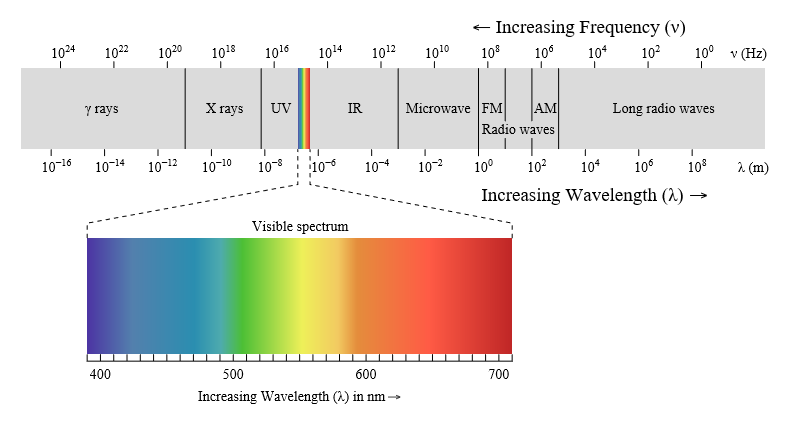
\includegraphics[width=\textwidth]{Includes/1-electromagnetic-spectrum.png}
        \caption{Electromagnetic spectrum}
        \label{fig:1-electromagnetic-spectrum}
    \end{figure}

    In the visual spectrum, usually reflected light is the measured. 
    In the infra-red spectrum (IR), light emitted from a certain wavelength is measured.
    This is because all bodies have a temperature above absolute zero, and this temperature is detectable as radiation.

    The IR spectrum goes from 1400 nm wavelenght to 1 mm and are further subdivided due to its width:


    \begin{itemize}
        \item  Short-wave infra-red (SWIR): 1,4 to 3,0 µm
        \item  Medium-wave infra-red (MWIR): 3,0 µm to 8 µm
        \item Long-wave infra-red (LWIR): 8 to 15 µm
        \item Far-infra-red (FIR): 15 µm to 1 mm
    \end{itemize}
    
    Like in the visual spectrum, TIR information is obtained in a purely passive way.
    Thermal infra-red detectors called bolometers are mostly used on drones or ground stations due to their small volume, weight, and energy consumption. 
    They offer a low accuracy in relative and absolute temperature measurement and are relatively inert, leading to a low ground resolution for moving systems (drones) but worthwhile for aircrafts with small payloads.     
    More complex systems are cooled to cryogenic temperatures to reduce thermal noise, a random electronic fluctuation which power depends linearly with the temperature and can interfere with the infrared signals. The noise reduction allows the sensor to have higher sensitivity and accuracy.
    In contrast to bolometers, they are significantly larger and require more energy, making them unsuitable for use on drones.
    These types of detectors are used on all common TIR satellite systems.

    \subsection{Land surface temperature}


        Land Surface Temperature (LST) is the radiative temperature of the land, derived from the previously mentioned thermal infra-red radiation that the Earth’s surface emits.

        It is one of the key parameters that affect surface energy balance, regional climates, heat fluxes, and energy exchanges.
        When taking Earth’s temperature, the interest relies in thermal infra-red (TIR) specifically, which has a wavelength of 3 to 14 µm (both MWIR and LWIR), corresponding to black body temperatures of between -60°C and 700 °C, according to Planck’s law.

        \begin{equation}
            B_{\lambda}(T) = \frac{C_1}{\lambda^5 \left[ \exp\left(\frac{C_2}{\lambda T}\right) - 1\right]},
        \end{equation}

        Where $B_{\lambda}(T)$ is the spectral radiance, $C_1$ and $C_2$ are physical constants, and $\lambda$ is the wavelength of the radiation. 
        Accurate LST retrieval from TIR data depends on atmospheric effects and sensor parameters such spectral range and viewing angle, and surface parameters such as emissivity and geometry. Many researchers have proposed different approaches for LST retrieval considering these factors.
        These algorithms are named considering the number of TIR bands used. For instance, single-channel or mono-window algorithms use one TIR band. However, split window or multi-channel methods include more than one TIR band. Some examples of these methods are Single Channel Algorithm (SCA) \cite{sca2009}, and Mono Window Algorithm (MWA) \cite{mwa2001}. The reader is referred to \cite{LI201314} for a more detailed review.


        A straightforward way to retrieve LST from a TIR band is inverting the simplified radiative transfer equation (RTE) \cite{becker90}. This equation contemplates the fact that the radiance measured by the sensor is a combination of the emitted radiance from the surface coming from an element that is not a blackbody, the reflected radiance from the atmosphere and the radiance emitted by the atmosphere itself.


        \begin{equation}
            \begin{aligned}
            L_{sensor} &= \left[ \varepsilon \cdot B_{\lambda}(T) + (1 - \varepsilon) \cdot L_{atm}^{\downarrow} \right] \tau + L_{atm}^{\uparrow} \\
            B_\lambda (T) &= \frac{L_{sensor} - L_{atm}^{\uparrow}- \tau (1 - \varepsilon) \cdot L_{atm}^{\downarrow}}{\varepsilon \tau} 
            \end{aligned}
        \end{equation}

        Where $L_{sensor}$ is the radiance measured by the sensor, $\varepsilon$ is the surface emissivity, $B_{\lambda}(T)$ is the Planck function, $L_{atm}^{\downarrow}$ is the downwelling path atmosphere radiance and $L_{atm}^{\uparrow}$ is the upwelling path atmosphere radiance. 
        The temperature can then be obtained from the spectral radiance by inverting the Planck's law:

        \begin{equation}
            T = \frac{C_2}{\lambda \cdot \log\left(\frac{C_1}{\lambda^5 \cdot \left[ \frac{L_{sensor} - L_{atm}^{\uparrow}- \tau (1 - \varepsilon) \cdot L_{atm}^{\downarrow}}{\varepsilon \tau}  \right]}+1\right)}
        \end{equation}

        From all the inputs for LST retrieval, radiance is the only one that is not available in high resolution, making it the bottleneck for the task. The high dependency between LST and TIR resolution makes them of particular interest for this work.
        
       

    \subsection{Quality dimensions of remote sensing data}

    Remote sensing data can be characterized by four quality dimensions, as stated in \cite{HORNING20082986}:

    \begin{itemize}
        \item Spatial resolution: This is often simply referred to as resolution and is the size of a pixel in ground dimensions. 
        In most cases an image's resolution is labeled with a single number, such as 30 m, which represents the length of a side of a square pixel if it were projected onto the Earth's surface.
        If the pixel were rectangular, then the length and width of the pixel would be provided.
        \item Spectral characteristics: This includes bandwidth, band placement, and the number of bands.
        Spectral bandwidth, or spectral resolution as it is often called, refers to the range of wavelengths that are detected in a particular image band.
        This is effectively a measure of how precisely an image band measures a portion of the EMS.
        Band placement defines the portion of the EMS that is used for a particular image band.
        For example, one band might detect blue wavelengths and another band might detect thermal wavelengths along the EMS.
        The last spectral variable is the number of bands. The more bands that are available the more precisely spectral properties of a feature can be measured.
        \item Acquisition dynamics: This has two components. The first is the minimum time a particular feature can be recorded twice, often called the revisit time or temporal resolution.
        Some sensors with a very wide field of view can acquire multiple images of the same area in the same day whereas some sensors have a repeat frequency of several weeks.
        The other component is the timing of the acquisitions. 
        Dynamic features such as forests shedding leaves in autumn and events such as flooding often have an optimum time for which they should be imaged.
        For example, the identification of deciduous vegetation is aided by acquiring imagery during leaf-on and during leaf-off periods.
        \item Sensitivity of the sensor: This is defined by the dynamic range of the sensor as well as the range of digital numbers that can be used to represent the pixel values.
        Sensors have lower limits below which a signal is not registered and upper limits above which the sensor saturates and is unable to measure increases in radiance.
        The detail that can be measured between these extremes is determined by the range between the minimum and maximum digital numbers permitted for a particular data type.
        This potential range of values is often referred to as quantization or radiometric resolution.
    \end{itemize}
    
    
    \newpage
    

\section{Motivation}

Advancements in satellite technology, particularly in thermal infra-red sensing, have emerged as a promising solution to monitor physical processes related to climate change such as water stress, evapotranspiration, wildfires or urban heat.
Unlike ground-based methods, satellites can continuously monitor vast tracts of land regardless of smoke or geographical barriers, providing critical real-time data that can significantly enhance early detection and response efforts. 
However, while current satellite systems offer extensive spatial coverage and consistent data collection, they are not without limitations, particularly in the quality dimension of spatial and temporal resolution.

Throughout this section, the main applications that OroraTech is working on are presented, as well as the thermal data products requirements that the literature has identified as vital for their development.
The trade-off between spatial and temporal resolution that the current available products will be further discussed, which is the main driver for super resolution.
    

    \subsection{Wildfire Monitoring}

    Forest fires can be natural or man-made phenomena that occurred in natural ecosystems and usually, they spread uncontrollably.
    The have increased steadily worldwide over the past decade, and according to the UN Environment Programme (UNEP), this trend will continue, with a potential 50\% increase in forest fires by the end of the century \cite{UNEP2021Wildfire}. 
    The escalating frequency and intensity of wildfires across the globe have prompted a reassessment of current monitoring systems and methodologies. Traditional ground and aerial surveillance methods are increasingly proving inadequate in the face of rapidly spreading, unpredictable fires, particularly those obscured by smoke and difficult terrain. This inadequacy hinders effective firefighting efforts and exacerbates the environmental, economic, and human toll of these disasters. 
    Luckily, in most cases, a layer of fume is not an obstacle for a satellite to detect a fire, as they rely on thermal infra-red sensors that can measure radiance through the smoke.

    Prevention is the most effective way to fight wildfires, and early detection is key to achieving this goal. 
    With timely access to thermal data from space, potential wildfires could be identified before they spread, minimizing damage and saving lives.
    Although satellite-based imagery is used by emergency response agencies to monitor large-scale wildfires that burn over extensive periods, the wait interval for a satellite overpass induces a considerable time delay, which prevents its application in time-sensitive fire detection scenarios, such as emergency evacuations, early detection or search-and-rescue operations \cite{lippitt2015time}. 

    OroraTech's looks to circumvent the overpass wait interval by launching a swarm of small satellites that have  been especially helpful for detecting newly born fires that started as a result of a bigger fire spreading, burning the material around its vicinity. The team develops its own sensors capable of providing up-to-date thermal data of the entire Earth every 30 minutes, starting from 2026.
    
    However, another parameter vital to measure fire risk, detect burn areas, and monitor vegetation recovery is the spatial resolution. The coarse spatial resolution that the smaller payloads these satellites provide does not enable the reliable detection of smaller fires. Additionally, higher spatial resolution is needed to better estimate the fire front, which is vital for the emergency response teams to plan their actions.
    Moreover, High resolution data has been used to validate characteristics of false positives in fire detection algorithms applied to low resolution scenes\cite{ijgi11120601}. 



    \subsection{Urban heat}

    Productivity losses due to heat currently cost an estimated \$100 billion annually only in the U.S alone.
    The U.K. experienced unprecedented temperatures too, temporarily knocking out services for giants like Google and Oracle and further affecting their clients.
    These are only a few examples of how businesses are affected by extreme temperatures in urban areas \cite{atlanticcouncil2021extreme}.  

    Public interest and concern about heat waves are steadily rising, especially in moderate climate areas such as North Europe. Heat waves are a major cause, specially in vulnerable population such as elderly people who are more prone to heat stress, pregnant individuals with difficulty adjusting to heat changes, outdoor workers who are exposed to extreme heat for prolonged periods and low-income neighborhoods with poor-quality buildings, between others \cite{Hsu2021Disproportionate}.   

    Urban heat refers to the phenomenon where urban areas experience higher temperatures than their more rural surroundings.
    This effect can be attributed to various factors such as building geometry, thermal properties of building materials, radiation properties of surfaces, and anthropogenic heat release from sources such as traffic and industry \cite{deilami2018urban}. 
    In particular,  the Urban Heat Island (UHI) phenomenon refers to the air temperature differences between urban areas and their surrounding rural regions, which is typically most pronounced during the evening and night hours. 

    Monitoring the UHI effect traditionally involves recording measurements from meteorological stations located in urban and rural areas throughout the region.
    However, an alternative method is to use thermal remote sensing, which allows for the monitoring of large areas without the need for multiple physical sensors placed throughout the city.
    Research suggests that a Ground Sampling Distance (GSD) of 50m to 100m is the minimum spatial resolution requirement for urban thermal environment studies \cite{mohamed2017land, sobrino2012impact, huang2013generating}. 
    This conditions can be met by missions such as Landsat \cite{USGS2023Landsat} and Terra \cite{terra_nasa}, which provide a high spatial resolution in the thermal infra-red band.
    However, their revisit time in the span of weeks severely limits the analysis of dynamic processes with a temporal resolution in the order of hours, such as the UHI. 

    Existing studies on the UHI effect have been limited by the low spatial resolution of the images used and the lack of satellite images available at different times of the day \cite{Zhu2021, Shi2019}. 
    In particular, researchers explicitly state their limitations \cite{Shi2019} due to the low frequency of revisits while studying the Park Cool Island (PCI) \cite{Yang2017} phenomenon. 
    The influence of vegetation cover on the urban heat island (UHI) phenomenon has been recognized as the foremost determinant \cite{deilami2018urban}, where parks have been found to exert a cooling impact.
    Fig. \ref{fig:1-skopie-UHI} illustrates an example that demonstrates this influence. 
    
    \begin{figure}[H]
        \centering
        \begin{minipage}{0.5\textwidth}
            \centering
            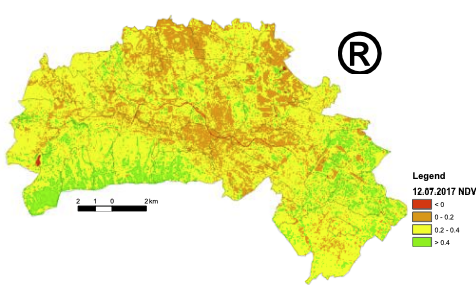
\includegraphics[width=\textwidth]{Includes/1-skopje-NDVI.png}
            \label{fig:1-skopje-NDVI}
        \end{minipage}\hfill
        \begin{minipage}{0.5\textwidth}
            \centering
            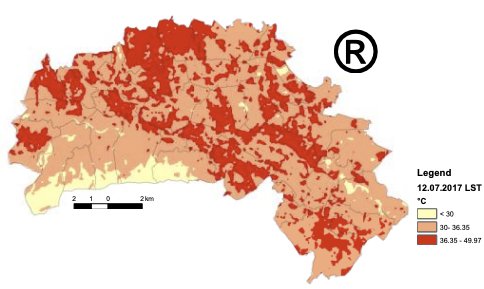
\includegraphics[width=\textwidth]{Includes/1-skopje-LST.png}
            \label{fig:1-skopje-LST}
        \end{minipage}
        \caption{Normalized Difference Vegetation Index \cite{Rouse1973MonitoringVS} and LST measurements for the zone of Skopje, North Macedonia. Urban areas with a lower vegetation index tend to have a higher temperature than their rural counterparts. Source : \cite{skopje2018}.} 
        \label{fig:1-skopie-UHI}
    \end{figure}

    Converting the low resolution images coming from private constellations into high-resolution images through post-processing techniques like super resolution could enable new frontiers in the study of urban heat. 


    \subsection{The spatio-temporal trade off}

        Sensors typically trade spatial resolution for temporal resolution and  it has been difficult historically to maximize both.
        Sensors that have a high spatial resolution often cover a smaller area than a sensor with lower spatial resolution.
        This is because with a smaller field of view, it takes longer to cover the same area. Thus, as spatial resolution increases, temporal resolution decreases.

        Essentially, it can be said that currently, the TIR data products that are used for developing LST data has either: 
        
        \begin{itemize}
            \item high temporal resolution (sub-daily images) but very low spatial resolution ( in the km range).
            \item High spatial resolution ( $<$ 100 m) but low temporal resolution (several days up to weeks).
        \end{itemize}

        The applications mentioned before have requirements in both spatial and temporal resolution. 
        The zone of interest, composed of sub-daily frequency and a GSD smaller than 100m, is not covered by any of the existing systems.
        Private missions, using smaller satellites, can leverage on constellations  to provide a higher temporal resolution.
        However, the spatial resolution is still limited by the payload mass and energy consumption constraints.
        This trade-off can be described by displaying the resolution of some of the LST/TIR data products available, as in Fig. \ref{fig:1-spatio-temporal-trade-off}. 

        \begin{figure}[H]
            \centering
            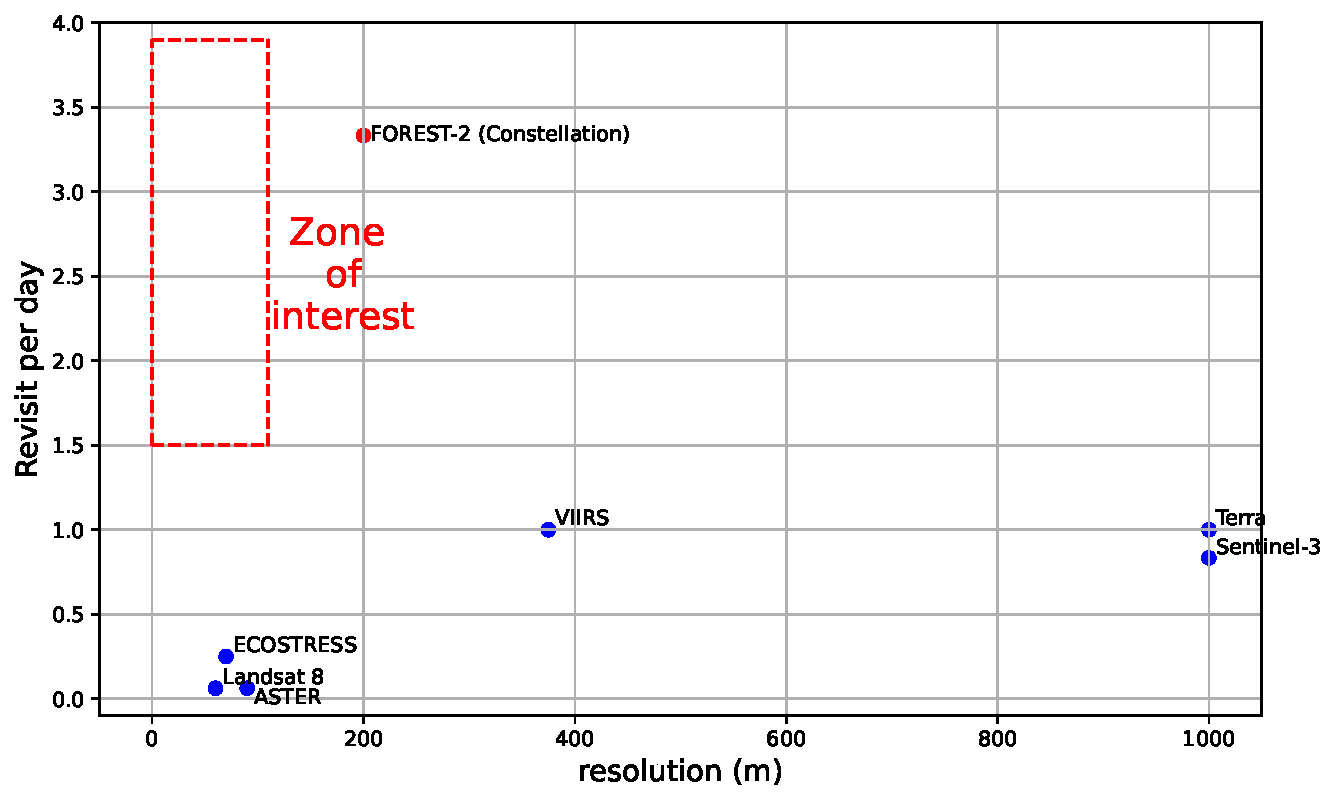
\includegraphics[width=\textwidth]{Includes/2-scatterplot-res-revisit.pdf}
            \caption{Scatter plot of the spatial and temporal resolution of some of the LST/TIR data products available.
                     The trade-off is evident, no mission can provide products in the zone of interest.
                     Constellations may help with temporal resolution, but the spatial resolution is still limited.}
            \label{fig:1-spatio-temporal-trade-off}
        \end{figure}

        This opens the question of whether it is possible to increase the spatial resolution of the data products available using a post-processing technique such as super resolution, without compromising the physical consistency of the scenes.
        The main techniques of super resolution and their most difficult challenges to apply them to LST/TIR data are described in the next section.

\newpage